\documentclass[12pt,letterpaper]{article}
\usepackage{graphicx,textcomp}
\usepackage{natbib}
\usepackage{setspace}
\usepackage{fullpage}
\usepackage{color}
\usepackage[reqno]{amsmath}
\usepackage{amsthm}
\usepackage{fancyvrb}
\usepackage{amssymb,enumerate}
\usepackage[all]{xy}
\usepackage{endnotes}
\usepackage{lscape}
\newtheorem{com}{Comment}
\usepackage{float}
\usepackage{hyperref}
\newtheorem{lem} {Lemma}
\newtheorem{prop}{Proposition}
\newtheorem{thm}{Theorem}
\newtheorem{defn}{Definition}
\newtheorem{cor}{Corollary}
\newtheorem{obs}{Observation}
\usepackage[compact]{titlesec}
\usepackage{dcolumn}
\usepackage{tikz}
\usetikzlibrary{arrows}
\usepackage{multirow}
\usepackage{xcolor}
\newcolumntype{.}{D{.}{.}{-1}}
\newcolumntype{d}[1]{D{.}{.}{#1}}
\definecolor{light-gray}{gray}{0.65}
\usepackage{url}
\usepackage{listings}
\usepackage{color}
\usepackage{float}

\definecolor{codegreen}{rgb}{0,0.6,0}
\definecolor{codegray}{rgb}{0.5,0.5,0.5}
\definecolor{codepurple}{rgb}{0.58,0,0.82}
\definecolor{backcolour}{rgb}{0.95,0.95,0.92}

\lstdefinestyle{mystyle}{
	backgroundcolor=\color{backcolour},   
	commentstyle=\color{codegreen},
	keywordstyle=\color{magenta},
	numberstyle=\tiny\color{codegray},
	stringstyle=\color{codepurple},
	basicstyle=\footnotesize,
	breakatwhitespace=false,         
	breaklines=true,                 
	captionpos=b,                    
	keepspaces=true,                 
	numbers=left,                    
	numbersep=5pt,                  
	showspaces=false,                
	showstringspaces=false,
	showtabs=false,                  
	tabsize=2
}
\lstset{style=mystyle}
\newcommand{\Sref}[1]{Section~\ref{#1}}
\newtheorem{hyp}{Hypothesis}

\title{Problem Set 4}
\date{Due: April 12, 2024}
\author{Applied Stats II}


\begin{document}
	\maketitle
	\section*{Instructions}
	\begin{itemize}
	\item Please show your work! You may lose points by simply writing in the answer. If the problem requires you to execute commands in \texttt{R}, please include the code you used to get your answers. Please also include the \texttt{.R} file that contains your code. If you are not sure if work needs to be shown for a particular problem, please ask.
	\item Your homework should be submitted electronically on GitHub in \texttt{.pdf} form.
	\item This problem set is due before 23:59 on Friday April 12, 2024. No late assignments will be accepted.

	\end{itemize}

	\vspace{.25cm}
\section*{Question 1}
\vspace{.25cm}
\noindent We're interested in modeling the historical causes of child mortality. We have data from 26855 children born in Skellefteå, Sweden from 1850 to 1884. Using the "child" dataset in the \texttt{eha} library, fit a Cox Proportional Hazard model using mother's age and infant's gender as covariates. Present and interpret the output.
\vspace{.25cm}

\noindent I load and inspect my data:

\lstinputlisting[language=R, firstline=41, lastline=53]{PS4.R}

\noindent I create the survival object \texttt{child\_surv} and, to further explore the data, plot the Kaplan-Meier curves for Overall Survival and across the two variables for Mother's Age \texttt{m.age} and Child's Sex \texttt{sex}, as shown in Figures 1-3.
\vspace{.25cm}

\noindent Note that on average, the expected survival probability for a child falls dramatically in their first few years of life, with the rate of decline gradually reducing up to age 15, at which point our data ends. Note the relatively tight margins along the KM curve, indicating relative stability in the estimated survivability of children over time.

\lstinputlisting[language=R, firstline=55, lastline=57]{PS4.R}
\lstinputlisting[language=R, firstline=85, lastline=93]{PS4.R}

\begin{figure}[!htpb]
	\centering
	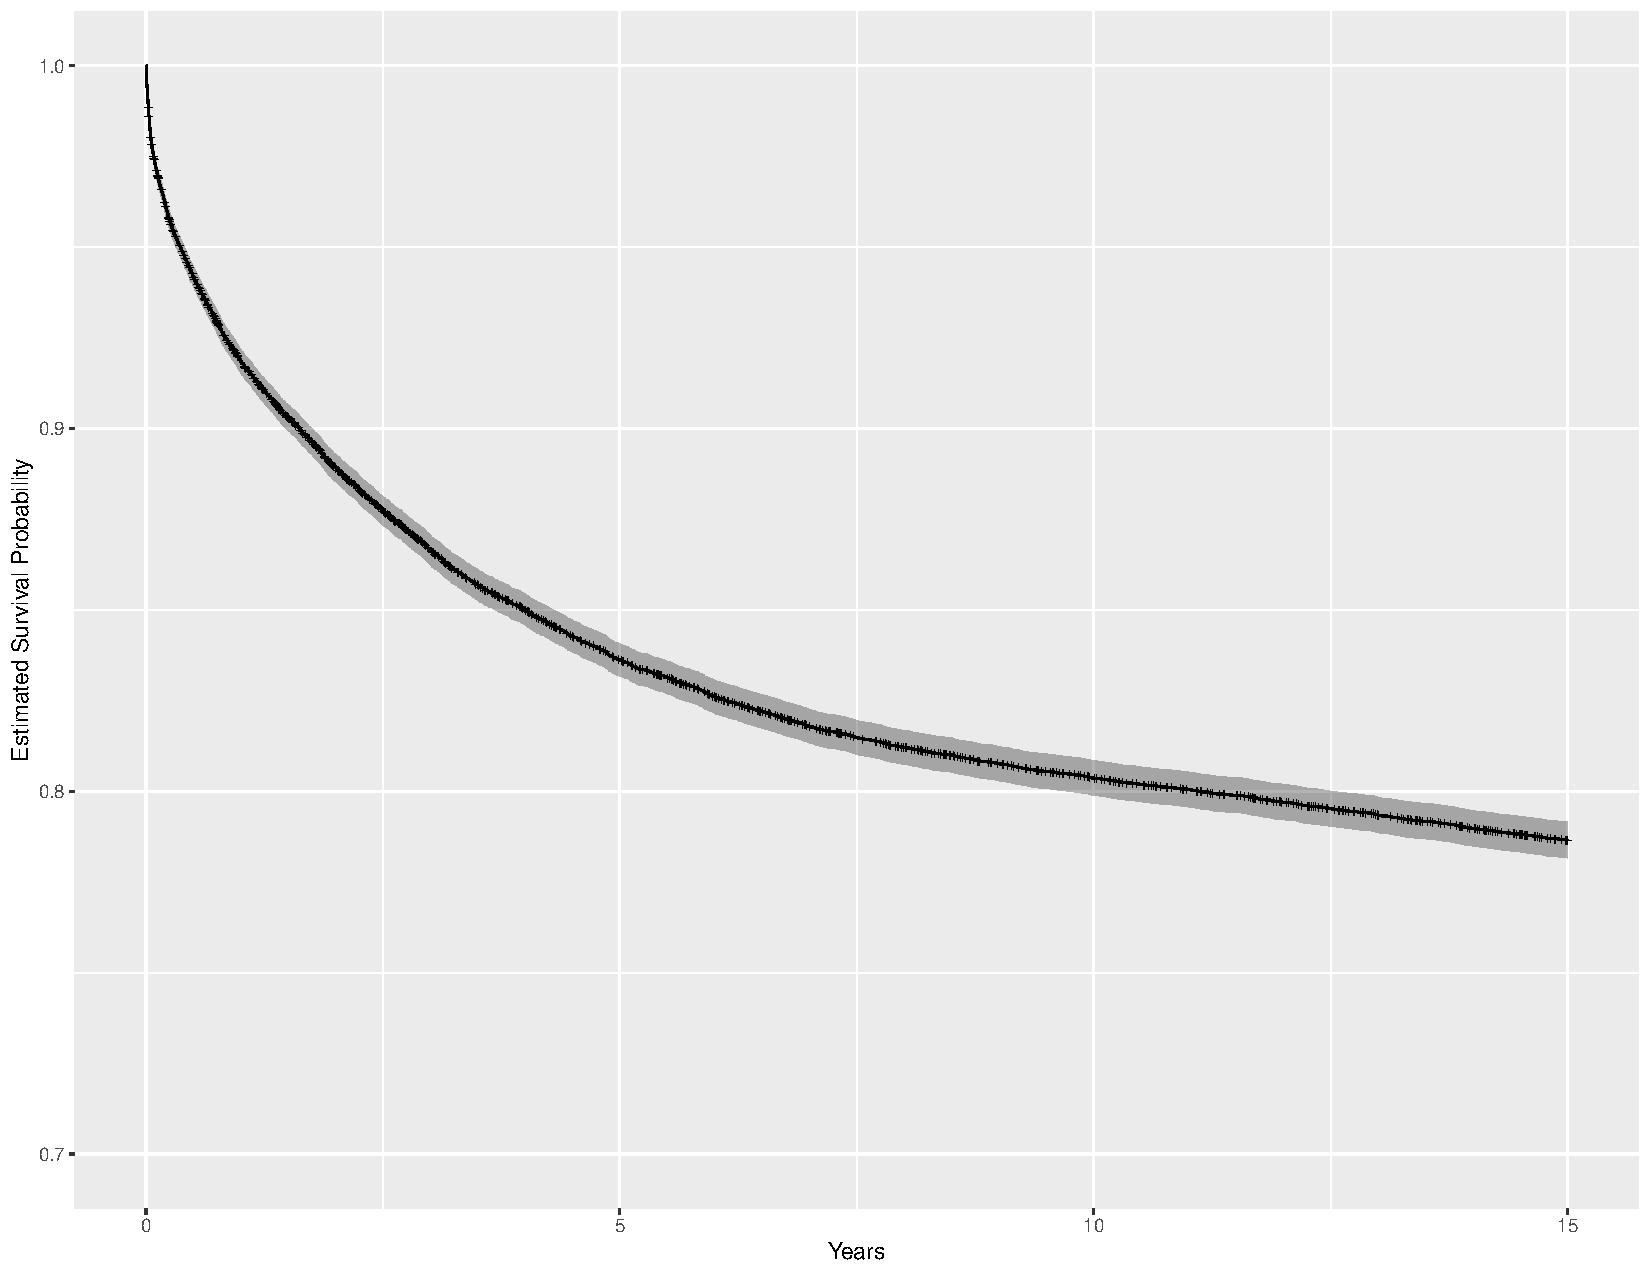
\includegraphics[width=0.8\textwidth]{overall.pdf}
	\caption{Kaplan-Meier Plot: Overall Survival Over Time}
	\label{fig:overall}
\end{figure}

\vspace{.25cm}
\noindent Note that Mother's Age is a continuous variable, and so for the purposes of plotting the KM curve, which requires a categorical predictor variable, I create a new object with variable \texttt{m.age\_bins}, which separates ages across five categories of approx. 10-years each (15-17, 18-24, 25-34, 35-44, and 45-51). Note the wide variation for the 15-17yrs - this is likely due to including a very small number of observations compared to the other age bands (see Table 1). That said, additional factors may affect the survivability outcomes for the children of especially young mothers, such as family connections, financial stability/socio-economic background of mother's parents, and the general health of a younger mother undergoing pregnancy and associated medical complications.

\lstinputlisting[language=R, firstline=63, lastline=81]{PS4.R}

\vspace{.25cm}

\noindent Excluding the 15-17yrs age group, on average, the mother's age appears to have a distinct effect on the estimated survival probability of the child, where children from younger mothers tend to have higher survival across all lived years, controlling for all other variables (though there is minor overlap in variation across lived years of the child).

\lstinputlisting[language=R, firstline=115, lastline=117]{PS4.R}

\begin{table}[!ht]
	\centering
	\begin{tabular}{cc}
		\hline
		Age Group & Freq \\ 
		\hline
		15-17 &  41 \\ 
		18-24 & 3876 \\ 
		25-34 & 13805 \\ 
		35-44 & 8512 \\ 
		45-54 & 340 \\ 
		\hline
	\end{tabular}
	\caption{Number of Mothers in Each Age Group}
\end{table}

\lstinputlisting[language=R, firstline=95, lastline=103]{PS4.R}

\begin{figure}[!htpb]
	\centering
	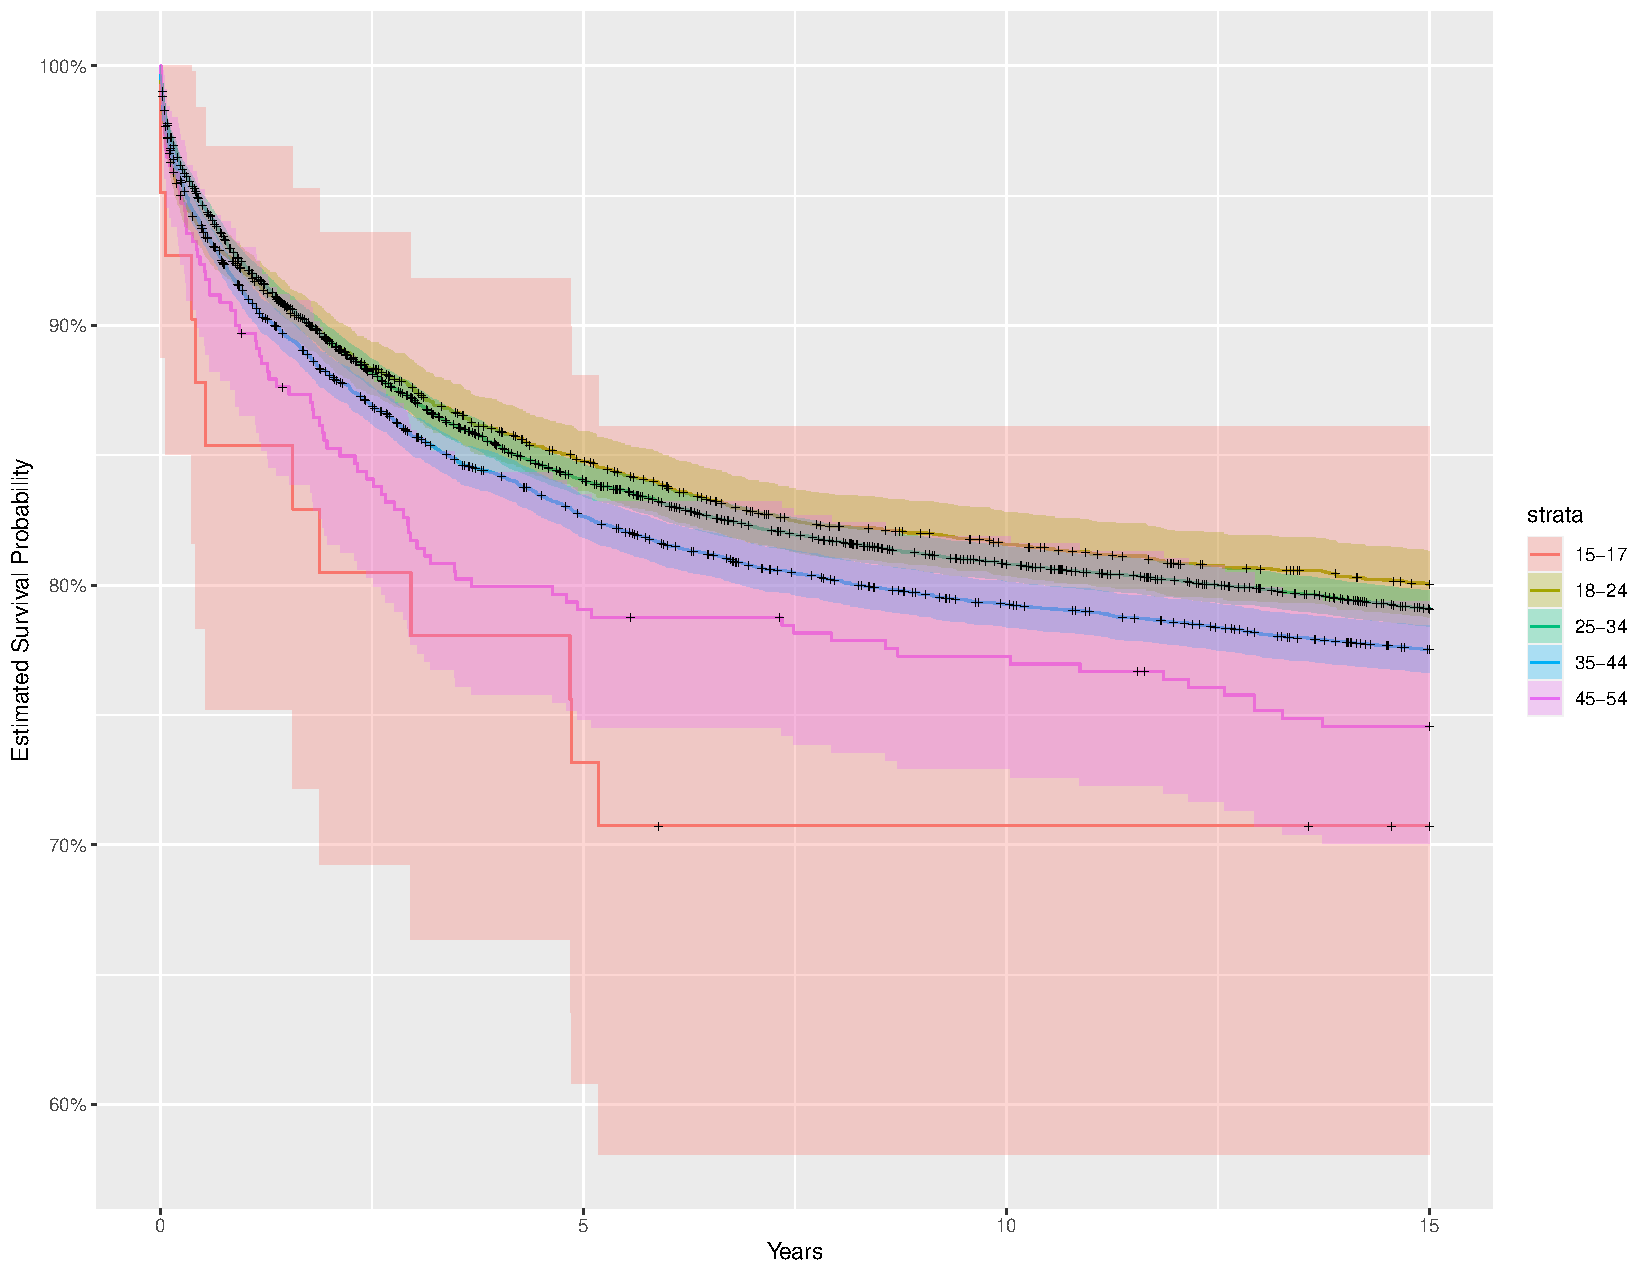
\includegraphics[width=0.8\textwidth]{age.pdf}
	\caption{Kaplan-Meier Plot: Mother's Age}
	\label{fig:age}
\end{figure}

\vspace{.25cm}
\noindent Note that Child's Sex appears to have a distinct effect on the (estimated) survival probability for the child - on average, females appear to have a higher probability of survival compared to males from birth and across all lived years, controlling for all other variables.

\lstinputlisting[language=R, firstline=105, lastline=113]{PS4.R}

\begin{figure}[!htpb]
	\centering
	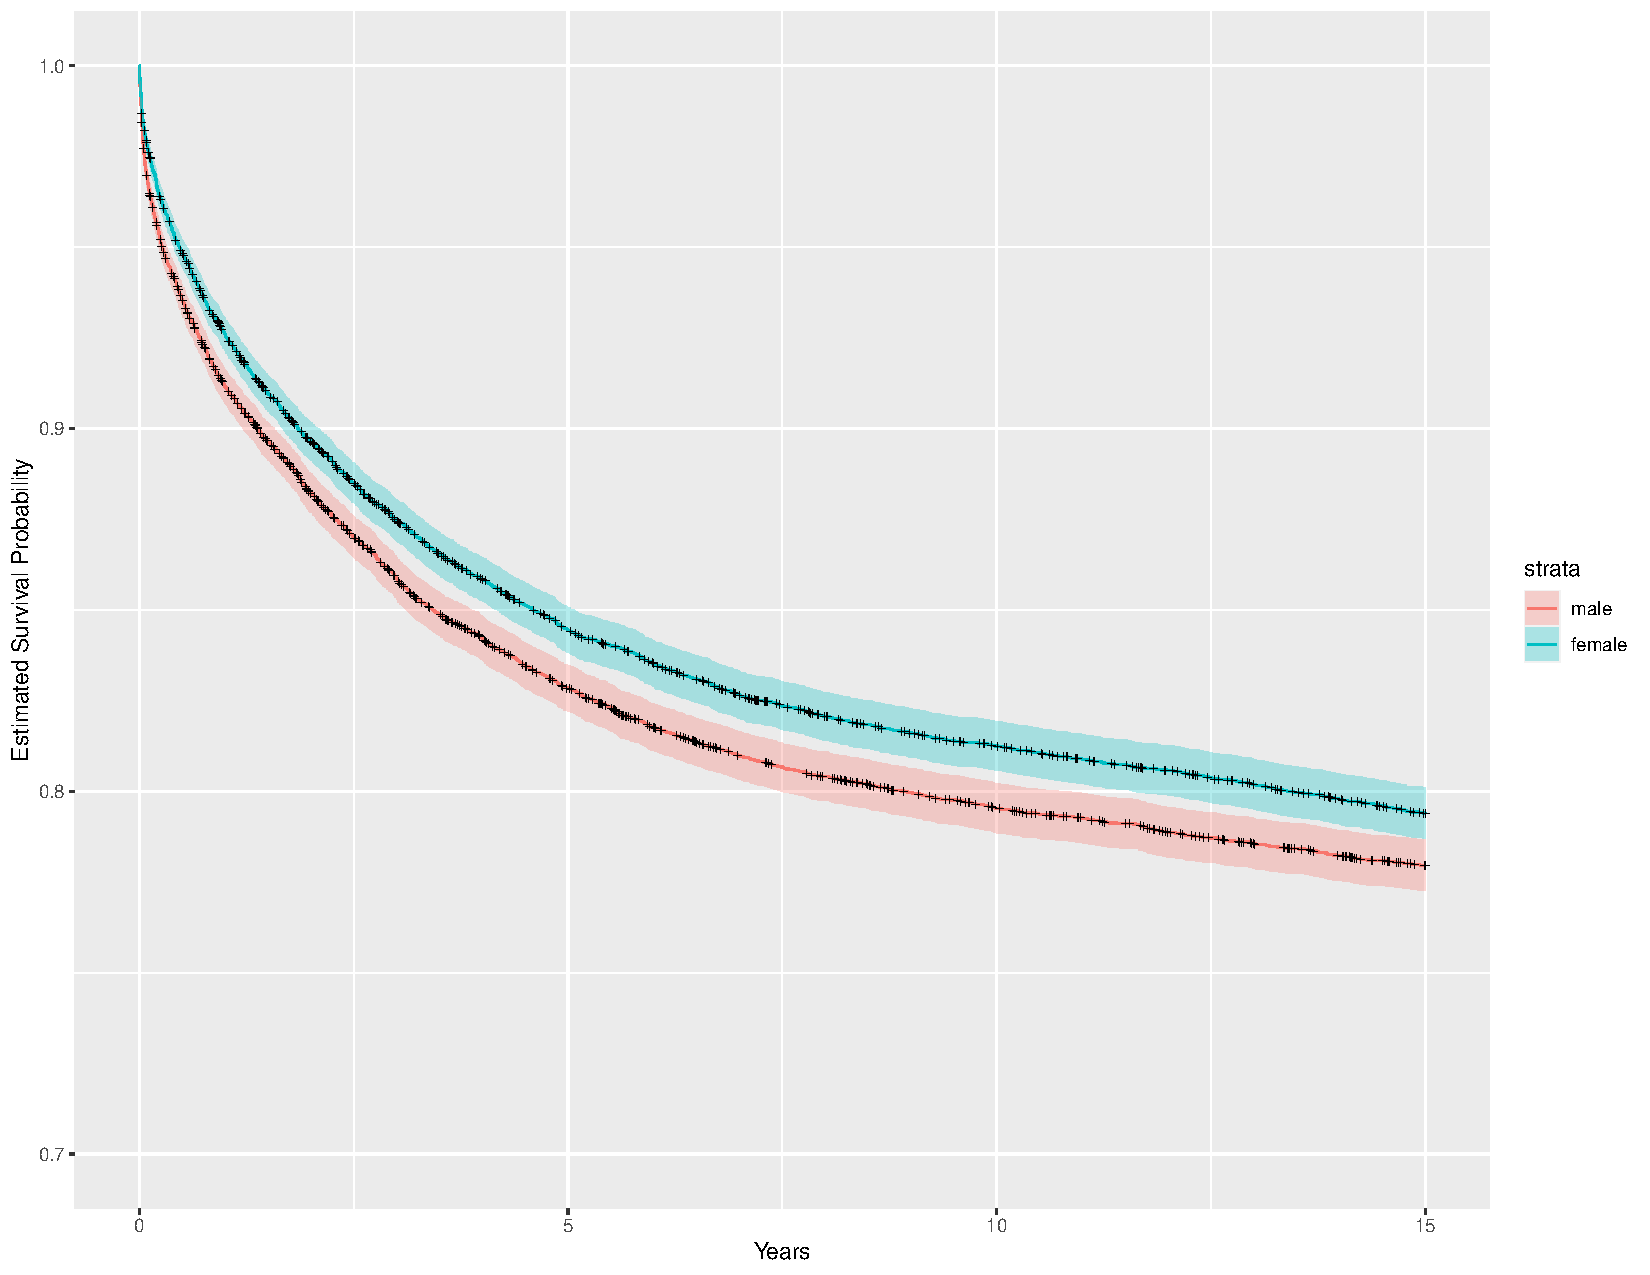
\includegraphics[width=0.8\textwidth]{sex.pdf}
	\caption{Kaplan-Meier Plot: Child's Sex}
	\label{fig:sex}
\end{figure}

\newpage
\noindent Next, I fit a Cox Proportional Hazard model using mother's age and infant's sex as covariates. I create two models - one additive and one interactive, to further explore the relationship between the two predictors and the survival probability of a child. Comparing both, we see the average partial effects on Survival Probability by Mother's Age and Child's Sex are statistically significant for the Additive model, while only Mother's Age is statistically significant in the Interaction model. They otherwise have the same or similar values in other notable figures on the table, and so I will continue with the additive model for further analysis.

\vspace{.25cm}

\noindent Regarding interpreting Table 2:
\begin{itemize}
	\item On average, for every 1-unit increase in the Mother's Age, the hazard (risk) of child survival increases by 0.008 units, holding all other variables constant. This estimate is statistically significant. In other words, on average, for every increase in 1 year in the Mother's Age, the child's probability of survivial decreases by 0.008 percentage points, holding all other variables constant.
	\item On average, a child who is female has a decreased hazard to their survival by 0.082 units, holding all other variables contant. This estimate is statistically significant. In other words, on average, children assigned female at birth have an average increase in 0.082 percentage points in comparison to children assigned male at birth, holding all other variables constant.
	\item The $R^2$ is 0.001, indicating that within the given data, the variations in Mother's Age and a Child's Sex co-vary with almost none of the variation in a child's estimated Survival Probability.
	\item The Wald Test is statistically significant, which gives evidence to reject the null hypothesis that no predictors included in the model have an effect on the outcome variable, and gives evidence for the alternative hypothesis that at least one of the included predictors - Mother's Age and/or Child's Sex - has an effect on a child's Estimated Survival Probability.
	\item The Score (Logrank) Test is statistically significant, which gives evidence to reject the null hypothesis that just the null model (mean) is better than the chosen model for estimating Survivability Probability for a child, and gives evidence for the alternative hypothesis that the chosen model is a better fit to the data on average.
\end{itemize}
\vspace{.25cm}
\noindent In conclusion, while there is significant evidence supporting the validity of this model, due to the oerall poor model fit of The $R^2$ = 0.001, another model or alternative explanatory variables may be more appropriate or useful for estimating the Survivability Probability of children born in Skellefteå, Sweden from 1850 to 1884.

\lstinputlisting[language=R, firstline=119, lastline=126]{PS4.R}

\begin{table}[!htbp]
	\centering
	\caption{Cox Proportional Hazard Model: Additive} 
	\label{} 
	\begin{tabular}{@{\extracolsep{3pt}}lc} 
		\\[-1.8ex]\hline 
		\hline \\[-1.8ex] 
		& \multicolumn{1}{c}{\textit{Dependent variable:}} \\ 
		\cline{2-2} 
		\\[-1.8ex] & child\_surv \\ 
		\hline \\[-1.8ex] 
		m.age & 0.008$^{***}$ \\ 
		& (0.002) \\ 
		& \\ 
		sexfemale & $-$0.082$^{***}$ \\ 
		& (0.027) \\ 
		& \\ 
		\hline \\[-1.8ex] 
		Observations & 26,574 \\ 
		R$^{2}$ & 0.001 \\ 
		Max. Possible R$^{2}$ & 0.986 \\ 
		Log Likelihood & $-$56,503.480 \\ 
		Wald Test & 22.520$^{***}$ (df = 2) \\ 
		LR Test & 22.518$^{***}$ (df = 2) \\ 
		Score (Logrank) Test & 22.530$^{***}$ (df = 2) \\ 
		\hline 
		\hline \\[-1.8ex] 
		\textit{Note:}  & \multicolumn{1}{r}{$^{*}$p$<$0.1; $^{**}$p$<$0.05; $^{***}$p$<$0.01} \\ 
	\end{tabular} 
\end{table} 

\begin{table}[!htbp!] \centering 
	\caption{Cox Proportional Hazard Model: Interaction} 
	\label{} 
	\begin{tabular}{@{\extracolsep{3pt}}lc} 
		\\[-1.8ex]\hline 
		\hline \\[-1.8ex] 
		& \multicolumn{1}{c}{\textit{Dependent variable:}} \\ 
		\cline{2-2} 
		\\[-1.8ex] & child\_surv \\ 
		\hline \\[-1.8ex] 
		m.age & 0.007$^{**}$ \\ 
		& (0.003) \\ 
		& \\ 
		sexfemale & $-$0.127 \\ 
		& (0.140) \\ 
		& \\ 
		m.age:sexfemale & 0.001 \\ 
		& (0.004) \\ 
		& \\ 
		\hline \\[-1.8ex] 
		Observations & 26,574 \\ 
		R$^{2}$ & 0.001 \\ 
		Max. Possible R$^{2}$ & 0.986 \\ 
		Log Likelihood & $-$56,503.430 \\ 
		Wald Test & 22.530$^{***}$ (df = 3) \\ 
		LR Test & 22.624$^{***}$ (df = 3) \\ 
		Score (Logrank) Test & 22.562$^{***}$ (df = 3) \\ 
		\hline 
		\hline \\[-1.8ex] 
		\textit{Note:}  & \multicolumn{1}{r}{$^{*}$p$<$0.1; $^{**}$p$<$0.05; $^{***}$p$<$0.01} \\ 
	\end{tabular} 
\end{table} 

\end{document}
